\section{Context and Motivation} \label{Introduction-Context}

% Internet of Things
\npara \textbi{Internet of Things} or \hyperref[Acronym-IoT]{IoT} has recently played an important role in connecting physical objects into the internet network.
The development of hardware capabilities and communication technologies allow an object or a \textit{thing} in our daily lives which is equipped with sensors or actuators to connect to the internet network.
This process turns them into smart objects that can interact with users or with other devices in order to observe a physical phenomenon and perform an interaction \citep{SEnviro}.

% Trust in General
\npara In human society, there might be a number of service providers offering services that we need.
When a person wants to interact or consume the service from another, it is necessary to know how \textbi{trustworthy} they are, before one can decide to choose and start an interaction.
The way to know this trustworthiness can be based on the experienced users' recommendations, as well as from the evaluation based on service quality.
This is to guarantee that the service will satisfy users and will not cause consequent failures.

% Trust in IoT
\npara In the same way, an \hyperref[Acronym-IoT]{IoT} device can also communicate with each other in order to consume or provide services.
Figure \ref{fig:SIoTLuigiA} from \cite{SIoTSocialStructure}'s work shows a comparison between the components of social networks in humans and digital objects.
Trustworthiness management is a component that is relevant to the relationship management in human social networks.
To ensure that the provided services are reliable and not leading to consequent failures, it is important to consume the services from trusted providers.
Despite the fact that \textbi{trust} is a subjective concept and differs on each individual agent, it can be influenced by a quantity value such as \textbi{reputation index} which is a social quantity property of an agent \citep{ComputationalModelTrust}.
In consequence, it is necessary for an \hyperref[Acronym-IoT]{IoT} system to have an architecture that allows the management of device \textit{reputation indices} in the system, so that the devices that consume a service can use the value to decide whether they would trust the provider before establishing a new connection.

\begin{figure}[hbt!]
  \centering
  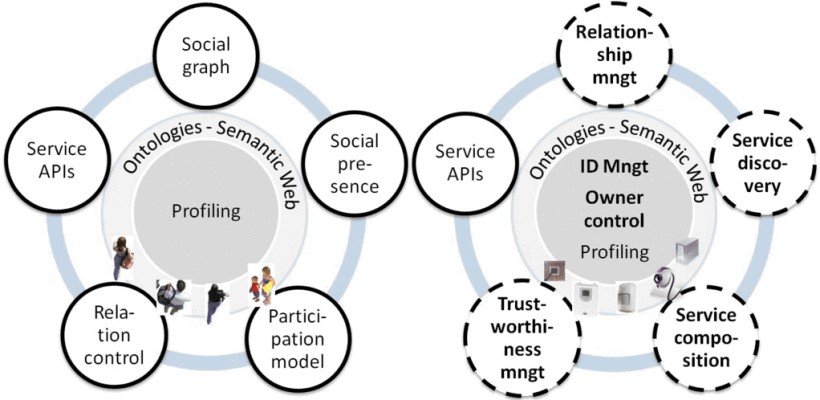
\includegraphics[width=\textwidth]{images/SIoTLuigiA.jpg}
  \caption{The components of social networks in human (left) and machines (right) \citep{SIoTSocialStructure}}
  \label{fig:SIoTLuigiA}
\end{figure}

% Area-based reputation
\npara Devices in an \hyperref[Acronym-IoT]{IoT} system are usually distributed over the geographical space and are able to move across different areas.
The location of the devices can be a factor that affects their trustworthiness \citep{TrustEnhancedSecurityLocationBased}.
For this reason, this master thesis will use this location component to build a reputation management system architecture to manage \hyperref[Acronym-IoT]{IoT} relationships.
In other words, it will include the spatial context of devices in order to establish the reputation values.

% Cloud-Fog-Edge architecture
\npara Another related technology is \textbi{cloud-fog-edge architecture}, which is a hierarchical architecture in the \hyperref[Acronym-IoT]{IoT}.
It divides the system into three layers which are \textit{cloud}, \textit{fog}, and \textit{edge} layer.
While the traditional cloud and edge layer were designed for heavy processing and low-level computation respectively, the fog layer was later proposed by Cisco to be an intermediate layer between these two layers \citep{CiscoUnleashFog}.
The capacity of a fog hardware is generally lower than the one in the cloud, but greater than edge devices enough so it can perform more complex calculations.
Hence, not all unnecessary computations have to be loaded in only cloud layer.
Moreover, the instalment of fog devices is also compromised in the extend between cloud and edge layers.
They are therefore generally geographically distributed, which are ideal to cover the location-based reputation management system.

% Blockchain
\npara The last related concept is \textbi{decentralisation}.
Due to the existence of fog layer, the intermediate devices are now distributed and not all computations need to be in the cloud layer.
\textbi{Blockchain} is a technology that allows data to be stored in a distributed way.
All nodes in a Blockchain network will share and possess the same data which are formed in blocks chronologically linked to each other like a chain.
The chain is distributed over the network which makes the system to be transparent and fault-tolerant \citep{BlockchainAdvantages}.
The Blockchain technology relies on hashing and consensus algorithms to confirm that all nodes in the network are having the same valid data, and it is not easy to tamper the chain.
The implementation of the Blockchain are well-known in \textbi{cryptocurrency}, such as Bitcoin and Ethereum.
But in the Ethereum, besides storing the money transactions it also allows \textbi{Smart Contract} which is an executable programme to be stored and callable from the Blockchain network.
In the other words, the Ethereum Blockchain network acts like a virtual machine that has the advantages of decentralisation in Blockchain.
Thus, this thesis proposes to adopt the Ethereum Smart Contract in the fog layer to create a decentralised application that is able to manage the reputation indices of an \hyperref[Acronym-IoT]{IoT} system.

\npara However, even the decentralised applications can execute any programming like a real computer does, but the characteristics of the Blockchain limit the ability of complex calculations in Smart Contracts.
Geometric spatial objects and their calculation which are related to complex algorithms and complicated data structures could cost an expensive computation in the Blockchain network.
For this reason, this thesis will use spatial indexing techniques in the implementation to study and challenge the possibility of manipulating spatial data in the Blockchain.
There are two hierarchical spatial indexing techniques being studied in this thesis.
The first one is \textbi{Geohash} which is an indexing technique invented by Gustavo Niemeyer \citep{GeohasUUID}.
And the second one is \textbi{S2} which was invented by Google engineers \footnote{\url{https://github.com/google/s2geometry}}.
Both techniques share the same hierarchical characteristics despite their different algorithms behind.
This thesis will therefore study the characteristics of these two techniques and compare their usage in the decentralised applications.

\section{Aims and Objectives} \label{Introduction-Aims}

\npara The main objective of this work is to propose a decentralised \hyperref[Acronym-IoT]{IoT} architecture which allows the location-based management of device services and their reputation values using Blockchain.

\npara To accomplish the main objective, this work will propose an \hyperref[Acronym-IoT]{IoT} architecture based on cloud-fog-edge structure, and decentralise the management system in the fog layer using the Ethereum Smart Contract.
Secondly, it will study and compare two spatial indexing techniques of Geohash and S2 which are used to represent the geographical data in the system, as well as implement and analyse their usage in the Smart Contracts.
Finally, it will simulate the architecture by implementing and deploying the system in the real \hyperref[Acronym-IoT]{IoT} devices.

\section{Research Questions} \label{Introduction-ResearchQuestions}

\begin{enumerate}
  \item \label{ResearchQuestion-DecentralisedFog} Is it possible to implement a decentralised area-based reputation management system of an IoT system in the fog layer using Blockchain?
  \item \label{ResearchQuestion-SpatialBlockchain} Is it possible to manipulate spatial data in a Blockchain network based on spatial indexing techniques?
  \item \label{ResearchQuestion-Geocoding} Comparing \textbi{Geohash} and \textbi{S2} geocoding techniques, which one does perform better in the proposed architecture, regarding speed, size, and suitability?
\end{enumerate}

\section{Document Structure} \label{Introduction-Structure}

\npara This thesis report is divided into five chapters.
The first chapter, \textbi{\nameref{Introduction}}, which is the current chapter, explains the motivation behind this work, the goals of the study, and the research questions.
Next chapter, \textbi{\nameref{Background}}, explains the related technologies and techniques.
There are three main topics related to this work, which are \textit{\nameref{Background-IoT}}, \textit{\nameref{Background-Blockchain}} and \textit{\nameref{Background-SpatialIndexing}}.
The third chapter, \textbi{\nameref{RelatedWorks}}, explores the literature of existing works that are related to the proposed architecture, as well as their technologies.
Fourthly, \textbi{\nameref{Methodology}}, explains the implementation design of this work.
It starts with the \textit{\nameref{Methodology-Architecture}} by introducing the whole picture of the proposed architecture, followed by the \textit{\nameref{Methodology-ExperimentDesign-Development}} which explains the tools and technologies used to develop the proposed architecture, and lastly, the \textit{\nameref{Methodology-ExperimentDesign}} elaborates the experimental procedures to test and evaluate the architecture.
After that, the fifth chapter of \textbi{\nameref{Results}} shows the development and experiment results of the architecture.
Followed by \textbi{\nameref{Conclusion}}, the last section which concludes the work and summarises experiment results, as well as suggests for the future development.
Finally, in the final part of the report, \textbi{\nameref{Appendix}} elaborates and explains related technologies and the data structures that could not be included in the previous chapters.
